\documentclass[tikz]{standalone}
\usetikzlibrary{patterns}
\usepackage{amsfonts}
\begin{document}
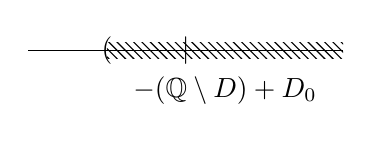
\begin{tikzpicture}

  \draw (-2, 0) -- (2, 0);
   \node at (-1, 0) {$($};
  \node at (0, 0) {$|$};
  \fill[pattern=north west lines] (-1, -0.1) rectangle (2, 0.1);
  \node at (0.5, -0.5) {$-(\mathbb Q \setminus D) + D_{0}$};

\end{tikzpicture}
\end{document}
